\chapter{Увод}

\label{Chapter1}

%----------------------------------------------------------------------------------------

\section{Актуалност на проблема и мотивация}

Разпознаването на изображения е способност на човека, която не е тривиално да бъде решена от компютър. Класифициране на изображения означава причисляване на изображение към един или повече класове с определена точност. Нека например имаме непресичащи се класове за превозни средства: автомобил, мотор, самолет, кораб, подовдница. Нека имаме изображенията, показани на \ref{fig:example_images}.\\[0.5cm]

\begin{figure}[h!]
\centering
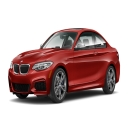
\includegraphics[width=115px,height=100px]{Figures/car.jpg}
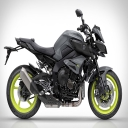
\includegraphics[width=115px,height=100px]{Figures/motorcycle.jpg}
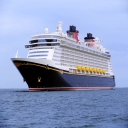
\includegraphics[width=115px,height=100px]{Figures/ship.jpg}
\caption{Примерни изображения}
\label{fig:example_images}
\end{figure}

Целта е първата картинка да се причисли към класа автомобили, втората към класа мотоциклети и третата към кораби. Това е елементарно за човешкото око, но компютърът вижда само последователност от нули и единици. Освен това при дадения пример разликите са големи, но може да се налага да се класифицират изображения, които са трудно различими дори с просто око.

Проблемът е особено актуален, поради непрестанното използване на социални мрежи и облачни услуги в световен мащаб. Всеки ден над 350 милиона снимки се качват само във Facebook \cite{FacebookFacts}. С използване на модерните технологии заснемаме гигантско количество изображения и много често след това просто забравяме за тях. Непосилна задача е ръчно да обозначим съдържанието на всяка една от снимките. Тук на помощ идва автоматичната обработка и анализ на съдържанието на изображения.

С намирането на добро решение на проблема са се захванали някои от най-големите компании в сферата на информационните технологии:

\begin{itemize}
\item \textbf{Google photos} \cite{GooglePhotos} използва автоматично класифициране на изображения, за да групира снимките, които качваме по категории и папки. Огромна публичност доби скандал с автоматичното категоризиране, при който двойка тъмнокожи бяха категоризирани като горили \cite{GoogleGorillas}. Това повдигна редица етични въпроси относно проблема. Google също предоставя и API за категоризация на изображения: Vision API \cite{GoogleVisionAPI}, което позволява интегрирането на софтуер за разпознаване на изображения в собствена система.
\item \textbf{Microsoft} също предоставя подобна услуга за своите облачни услуги. Те имат и аналогично API \cite{MicrosoftVisionAPI}.
\item Amazon, Dropbox също поддържат подобни услуги, което говори за потенциала на разпознаването на изображения.
\end{itemize}

Бизнесът на някои компании изцяло лежи на разпознаването на изображения. Такива са Imagga \cite{Imagga}, Clarifai \cite{Clarifai}.

Предоставянето на тази функционалност като услуга за бизнесите предразполага раждането на много оригинални идеи. Такива са вече споменатите облачни услуги. С наличието на API за разпознаване на изображения всеки доставчик на облачни услуги може да направи автоматична категоризация на изображенията на потребителите. Друг интересен случай са сайтове и приложения за споделяне на авторски изображения. При тях обемът на данните е огромен и в повечето случаи няма никаква конкретна информация.

Разпознаването на обекти в изображението би могло да бъде от полза и по отношение на сигурността. При голямо количество съдържание може лесно да се намерят например оръжия или снимки с нецензурирано съдържание. Обемът на снимките расте с гигантски размери и е единствено въпрос на въображение от страна на компаниите какви ползи могат да се извлекат от автоматичното категоризиране на изображения.

\section{Цел и задачи на дипломната работа}
Целта на дипломната работа е да проучи съвременните подходи за класифицирането на изображения, като се дават детайли за използването на конволюционни невронни мрежи с дълбоко обучение.

Задачите биха могли да се обобщят по следния начин:
\begin{enumerate}
\item Обзор на проблемната област. Да се направи проучване на различните софтуерни платформи, които може да се използват за класифициране на изображения в големи мащаби. Какви са предимствата и недостатъците на всяка една от тях. Какво използват най-големите компании в тази сфера.
\item Какви са условията (финансови, хардуерни и др.), за да построим класификатор с добра точност. Какво е добра точност и каква точност постигат готовите решения.
\item Подбор на данни за обучение. Намиране на достатъчно голям обем категоризирани изображения с добро качество с цел обучение.
\item Реализация на прототип за класификация на изображения.
\item Експерименти за оценка на точността на класификацията и възможностите за работа с големи данни.
\item Анализ на получените резултати.
\end{enumerate}

\section{Структура на дипломната работа}

Глава 1 е въведение в проблемната област. Тя цели да покаже кратко каква е целта на дипломната работа и мотивацията да се разреши точно този проблем. Обсъдени са резултатите, които трябва да се постигнат.

Глава 2 представя в детайли използваните алгоритми и подходи. Освен това в нея се аргументира изборът на подход с конволюционни невронни мрежи и се прави подробен анализ на най-доброто решение до момента на писане на дипломната работа.

Глава 3 мотивира избора на технологии, платформи, услуги и библиотеки, които са необходими при разработването на конволюционната невронна мрежа за класифициране на изображения. Направено е въведение в спецификите на Python и Tensorflow като са анализирани различните функционалности и спрямо изискванията на конкретния проблем е избрано подмножество от тях.

Глава 4 дава подробен поглед върху процеса по реализация на конволюционната невронна мрежа за класифициране на изображения и избора на архитектура. Вниманието е насочено към направените експерименти и анализ на резултатите от тях.

Глава 5 е заключителната част, даваща насоки за бъдещо развитие на системата и обобщаващо в каква степен са изпълнени първоначалните поставени цели и задачи. 
